\section{Posets of graph rewriting events}

\subsection{From transition systems to posets}

\begin{lemma}
  \label{lemma:pos_infl}
  Let $TS = (Q,R,E,T,I,<,\dashv)$ be a transition system and let $e,e' \in E$.
  \begin{enumerate}
  \item $e< e'\implies \labl(e)\xrightarrow{+}\labl(e')$;
  \item $e\dashv e' \implies\labl(e)\xrightarrow{-}\labl(e')$.
  \end{enumerate}
\end{lemma}
\begin{proof}
  \begin{enumerate}
  \item From~\autoref{def:seq_dep} $e_1 < e_2$ implies there exists two transitions $M\overset{m_1,p_1}{\Rightarrow} M_1$ and $M_1\overset{m_2,p_2}{\Rightarrow} M_2$ that are sequential dependent. For any such pair of transitions, using~\autoref{lem:completeness_causal_pair} there exists a causal pair which in turns implies that $\labl(e)\xrightarrow{+}\labl(e')$.

  \item From~\autoref{def:inhibition} $e_1 \dashv e_2$ implies there exists transition $M\overset{m_1,p_1}{\Rightarrow} M_1$ inhibiting transition $M\overset{m_2,p_2}{\Rightarrow} M_2$. For any such pair of transitions, using~\autoref{lem:completeness_inhib_pair} there exists an inhibiting pair which in turns implies that $\labl(e)\xrightarrow{-}\labl(e')$.
  \end{enumerate}
\end{proof}

\begin{remark}
  Sequential dependence (~\autoref{def:seq_dep}) is not transitive. Therefore when considering posets in~\autoref{def:poset}, we need to distinguish between the \emph{immediate} order relation and its transitive closure.
\end{remark}

\begin{definition}[Abstraction on a trace]
  \label{def:abstraction}
  Let $\Theta$ be a set of traces and let $\theta:M_0\overset{m_1,p_1}{\Rightarrow} M_1\overset{m_2,p_2}{\Rightarrow} M_2 \cdots \overset{m_n,p_n}{\Rightarrow} M_n$ be a trace in $\Theta$. Define $\alpha:\Theta\to\mathcal{S}$ an \emph{abstraction} function that maps a trace into a poset as follows:
  \begin{itemize}
  \item given a transition $M\overset{m,p}{\Rightarrow} M'$ define the \emph{abstract event} $e$ associated to it
    \[
    \alpha(M\overset{m,p}{\Rightarrow} M') = e
    \]
    such that $\labl(e) = p$.
  \item define a poset from a trace $\alpha(\theta) = (E,<,\labl)$ such that $\alpha$ is a bijection between transitions and abstract events and such that the sequential dependence between transitions is preserved:
    \begin{align*}
      \alpha(t_i:M_{i-1}\overset{m_{i},p_{i}}{\Rightarrow}M_i) = e_i \\
      e_i < e_j \iff t_i < t_j \text{ and } \alpha(t_i)=e_i, \alpha(t_j)=e_j
    \end{align*}
  \end{itemize}
\end{definition}

\begin{definition}[Set of posets]
  Let $TS = (Q,R,E,T,I,<,\dashv)$ be a transition system and let $\Theta = \{\theta_1,\cdots,\theta_n\}$ be a set of traces of $TS$.
  Define the set of posets obtained by abstraction on $\Theta$ as follows
  \[
  \alpha(\{\theta_1,\cdots,\theta_n\}) = (s_1,\cdots, s_k)\text{ with }k\leq n
  \]
  where for each poset $s = (E,\tleq,\labl)$ there exists at least one trace $\theta\in\Theta$ such that $\alpha(\theta) = (E,<,\labl)$ and where $\tleq$ is the reflexive and transitive closure of $<$.
%  A \emph{story} of TS, $s$ $=$ $(E_s,<_s)$, is a subset of events $E_s\subseteq E$ equipped with a binary relation on events $<_s$ which is the restrictions of $<$ to the set $E_s$.
\end{definition}

Henceforth the set of posets $\mathcal{S}$ stands for the set defined above.

%Instead of working on the transition system, we interpret ou logic over a set of stories, $\mathcal{S}$ with the constraint that $\mathcal{S}$ is closed under set inclusion: $s\in \mathcal{S} \implies \forall s'\subset_{\labl} s, s'\in\mathcal{S}$. We equip the set of stories $\mathcal{S}$ with the binary relation $\dashv_{\mathcal{S}}$, which is the restriction of $\dashv$ to the set of events $\cup_{s\in\mathcal{S}} E_s$.

%We are not interested in the extraction mechanism, as long as the identity of events and the relationships between them (causality and inihibition) are preserved.

%In the following subsection we define the \emph{concretisation} function.

\subsection{Refinement of graph rewriting rules}

In a poset of $\mathcal{S}$, we have that for any event, its immediate causes have a positive influence on it (\autoref{lemma:pos_infl}).

\begin{definition}[Decorate posets with the positive influence]
   Given a set of events $E$ and a labeling function $\labl$ on events, define a function $\mathit{decorate}:E\times E \to E\times E\times G$ that associates to a pair of events $(e,e')$ the following set
    \[
    \mathit{decorate}(e,e') = \{(e,e',O) : O\text{ is a graph such that }\labl(e)\redl{+}_O e'\}.
    \]

    Let $s = (E,<,\labl)$ be a poset. Define $\mathit{decorate}$ a function that sends a poset $s$ into a set of posets as follows
    \[
    \mathit{decorate}(E,<,\labl) =\{(E,\sqsubset,\labl) : e\sqsubset_O e' \iff (e,e',O)\in\mathit{decorate}(e,e')\text{ and }
    e<e'\}.
    \]
\end{definition}

Let us first give an example of a refinement of a poset and then introduce all notions we need formally.
\begin{example}
\label{ex:e1e2e3}
Let us consider the poset $(\{e_1,e_2,e_3,e_4\},\sqsubset)$ where $e_1\sqsubset_{O_1}e_2\sqsubset_{O_2}e_3$, $e_4\sqsubset_{O_4}e_3$ and $\labl(e_1)=r_1$, $\labl(e_2)=r_2$, $\labl(e_3)=r_3$, $\labl(e_4)=r_4$.

First we refine $r_2$ using the relation $r_1\redl{+}_{O_1} r_2$, (as we have seen in~\autoref{def:low_res}):
\[
\begin{tikzpicture} %[scale=0.8]
  \node (o1) at (0,-1) {\(O_1\)};
  \node (m1) at (0,1) {\(M_1\)};
  \node (n1) at (2,1) {\(N_1\)};
  \node (r1) at (-1,0) {\(R_1\)};
  \node (l1) at (-2.5,0) {\(L_1\)};
  \node (l2) at (1,0) {\(L_2\)};
  \node (r2) at (2.5,0) {\(R_2\)};
  \draw [->] (o1) -- (r1);
  \draw [->] (o1) -- (l2);
  \draw [->] (r1) -- (m1);
  \draw [->] (r2) -- (n1);
  \draw [->] (l2) -- (m1);
  \draw [vecArrow] (l1) -- (r1);
  \draw [vecArrow] (m1) -- (n1);
  \draw [vecArrow] (l2) -- (r2);
\end{tikzpicture}
\]
We apply a rewriting step to $M_1$ using rule $r_2$ to obtain $N_2$. We refine then $r_3$ using $N_2$ (this step is formally defined in~\autoref{def:seq_comb}):
\[
\begin{tikzpicture} %[scale=0.8]
  \node (o1) at (0,-1) {\(O_1\)};
  \node (m1) at (0,1) {\(M_1\)};
  \node (r1) at (-1,0) {\(R_1\)};
  \node (l1) at (-2.5,0) {\(L_1\)};
  \node (l2) at (1,0) {\(L_2\)};
  \node (r2) at (2.5,0) {\(R_2\)};
  \node (o2) at (3.5,-1) {\(O_2\)};
  \node (l3) at (4.5,0) {\(L_3\)};
  \node (r3) at (6,0) {\(R_3\)};
  \node (m2p) at (2.5,1) {\(N_1\)};
  \node (n) at (3.5,2) {\(M_2\)};
  \node (n2) at (5,2) {\(N_2\)};
  \draw [->] (o1) -- (r1);
  \draw [->] (o1) -- (l2);
  \draw [->] (r1) -- (m1);
  \draw [->] (l2) -- (m1);
  \draw [->] (o2) -- (r2);
  \draw [->] (o2) -- (l3);
  \draw [->] (l3) -- (n);
  \draw [->] (m2p) -- (n);
  \draw [->] (r2) -- (m2p);
  \draw [->] (r3) -- (n2);
  \draw [vecArrow] (l1) -- (r1);
  \draw [vecArrow] (l2) -- (r2);
  \draw [vecArrow] (l3) -- (r3);
  \draw [vecArrow] (m1) -- (m2p);
  \draw [vecArrow] (n) -- (n2);
\end{tikzpicture}
\]
Let us now integrate $e_4\sqsubset_{O_4} e_3$ in the sequence. Let $R_4\lemb M_3\remb L_3$ be the cospan obtained from $\labl(e_4)\redl{+}_O\labl(e_3)$.
We combine $M_2$ and $M_3$ using $L_3$ (concurrent combinator is formally introduced in~\autoref{def:conc_comb}):
\[
\begin{tikzpicture} %[scale=0.8]
  \node (l4) at (0.5,0) {\(L_4\)};
  \node (r4) at (2,0) {\(R_4\)};
  \node (o4) at (3,-1) {\(O_4\)};
  \node (m4) at (3,1) {\(M_3\)};
  \node (l3) at (4,0) {\(L_3\)};
  \node (r3) at (5.5,0) {\(R_3\)};
  \node (m2p) at (5,1) {\(M_2\)};
  \node (n) at (4,2) {\(M_4\)};
  \draw [->] (o4) -- (r4);
  \draw [->] (o4) -- (l3);
  \draw [->] (r4) -- (m4);
  \draw [->] (l3) -- (m4);
  \draw [->] (m4) -- (n);
  \draw [->] (m2p) -- (n);
  \draw [->] (l3) -- (m2p);
  \draw [vecArrow] (l4) -- (r4);
  \draw [vecArrow] (l3) -- (r3);
\end{tikzpicture}
\]
Lastly we have to propagate $M_4$ backwards to events $e_1$, $e_2$ and $e_4$.
\[
\begin{tikzpicture} %[scale=0.8]
  \node (o1) at (0,-1) {\(O_1\)};
  \node (m1) at (0,1) {\(M_1\)};
  \node (r1) at (-1,0) {\(R_1\)};
  \node (l1) at (-2.5,0) {\(L_1\)};
  \node (l2) at (1,0) {\(L_2\)};
  \node (r2) at (2.5,0) {\(R_2\)};
  \node (o2) at (3.5,-1) {\(O_2\)};
  \node (l3) at (4.5,0) {\(L_3\)};
  \node (r3) at (6,0) {\(R_3\)};
  \node (n1) at (2.5,1) {\(N_1\)};
  \node (m2) at (3.5,2) {\(M_2\)};
  \node (n2) at (6,2) {\(N_2\)};
  \node (m6) at (-2.5,3) {\(M_6\)};
  \node (m5) at (0,3) {\(M_5\)};
  \node (m4) at (3.5,3) {\(M_4\)};
  \node (n4) at (6,3) {\(N_4\)};
  \draw [->] (o1) -- (r1);
  \draw [->] (o1) -- (l2);
  \draw [->] (r1) -- (m1);
  \draw [->] (l2) -- (m1);
  \draw [->] (o2) -- (r2);
  \draw [->] (o2) -- (l3);
  \draw [->] (l3) -- (m2);
  \draw [->] (n1) -- (m2);
  \draw [->] (r2) -- (n1);
  \draw [->] (r3) -- (n2);
  \draw [vecArrow] (l1) -- (r1);
  \draw [vecArrow] (l2) -- (r2);
  \draw [vecArrow] (l3) -- (r3);
  \draw [vecArrow] (m1) -- (n1);
  \draw [vecArrow] (m2) -- (n2);
  \draw [->] (n2) -- (n4);
  \draw [->] (m2) -- (m4);
  \draw [->] (m1) -- (m5);
  \draw [->] (l1) -- (m6);
  \draw [vecArrow] (m4) -- (n4);
  \draw [vecArrow] (m4) -- (m5);
  \draw [vecArrow] (m5) -- (m6);
\end{tikzpicture}
\]
The refinement of our poset is then the set of transitions
\[
\begin{tikzpicture} %[scale=0.8]
  \node (m6) at (0,1) {\(M_6\)};
  \node (m5) at (1.5,1) {\(M_5\)};
  \node (m4) at (3,1) {\(M_4\)};
  \node (n4) at (4.5,1) {\(N_4\)};
  \node (m7) at (1.5,0) {\(M_7\)};
  \draw [vecArrow] (m4) -- (n4);
  \draw [vecArrow] (m5) -- (m4);
  \draw [vecArrow] (m6) -- (m5);
  \draw [vecArrow] (m7) -- (m4);
\end{tikzpicture}
\]
where $M_7$ is obtained by a rewriting of $M_4$ using rule $r_4$.
\end{example}

\begin{definition}[Refinement of a rule~\cite{information_carriers}]
  Let $r:L{\Rightarrow} R$ be a rule and let $m:L\emb M$ be a matching in a graph $M$. The production $M\Rightarrow N$ obtained by DPO rewriting of $M$ using the rule $r$ is called a \emph{refinement} of $r$.
\end{definition}

\begin{definition}[Refinement of a poset]
  Given a poset $s=(E,<,\labl)$ of graph rewriting events, the \emph{refinement} of $s$, is a bijection $\imath$ between events $e\in E$ and transitions $M\overset{m,p}{\Rightarrow} M'$ such that
  \begin{itemize}
  \item labels are preserved, i.e. $\labl(e)=p$;
  \item for all $e_1,e_2\in E$, if $e_1<e_2$ and $\imath(e_1) = M_1\overset{m_1,p_1}{\Rightarrow} M_1'$, $\imath(e_1) =M_2\overset{m_2,p_2}{\Rightarrow} M_2'$ then $M_1'\iso M_2$.
  \end{itemize}
\end{definition}

%Before giving the construction of a refinement $(M_i\overset{m_i,p_i}{\Rightarrow} M_{i+1})_{e_i\in E}$ let us first introduce some combinators of contexts.

%% \begin{definition}[Propagate a context]
%%   \label{def:propagate}
%%   Given a sequence $M_1{\Rightarrow} M_2\cdots {\Rightarrow} M_n\cdots {\Rightarrow} M_{m}$ and a graph $M_{n}'$ with $M_n\emb M_{n}'$ define the \emph{propagation} of $M_{n}'$ as the sequence  $M_1'{\Rightarrow} M_2'\cdots {\Rightarrow} M_n'\cdots {\Rightarrow} M_{m}'$ where
%%   \begin{itemize}
%%   \item $M_i'$, for $i<n$, is obtained by the reverse of the production $M_i\Rightarrow M_{i+1}$ applied to the new contexts;
%%   \item $M_i'$, for $n<i\leq m$, is obtained by the production $M_i\Rightarrow M_{i+1}$ applied to the new contexts.
%%   \end{itemize}
%% \end{definition}

\begin{definition}[Sequential combinator]
\label{def:seq_comb}
  Let $M\Rightarrow N$ and $L\Rightarrow R$ be two productions such that there exists $N\lemb O \remb L$ a cospan.
  \[
  (M\Rightarrow N)\oplus_O (L\Rightarrow R) = M'\Rightarrow N'
  \]
  where $N\emb M' \remb L$ is the pushout of the cospan $N\lemb O \remb L$ and $N'$ is obtained by a DPO rewriting of $M'$ by the production $L\Rightarrow R$.
  \[
  \begin{tikzpicture} %[scale=0.8]
    \node (o) at (0,-1) {\(O\)};
    \node (mp) at (0,1) {\(M'\)};
    \node (m) at (-2.5,0) {\(M\)};
    \node (n) at (-1,0) {\(N\)};
    \node (l) at (1,0) {\(L\)};
    \node (r) at (2.5,0) {\(R\)};
    \node (np) at (2,1) {\(N'\)};
    \draw [->] (o) -- (n);
    \draw [->] (o) -- (l);
    \draw [->] (n) -- (mp);
    \draw [->] (l) -- (mp);
    \draw [->] (r) -- (np);
    \draw [vecArrow] (m) -- (n);
    \draw [vecArrow] (l) -- (r);
    \draw [vecArrow] (mp) -- (np);
  \end{tikzpicture}
  \]
\end{definition}

\begin{definition}[Wide pushout~\cite{wide}]
The wide pushout of a family of morphisms $(L\to M_i)_i$ consists of a graph $M$ and a family of morphisms $(M_i\to M)_i$ such that the diagram commutes
\[
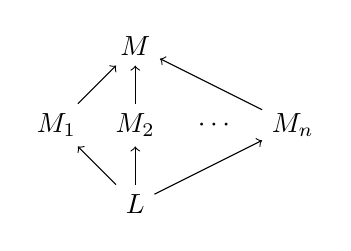
\begin{tikzpicture} %[scale=0.8]
  \node (o) at (0,-1) {\(L\)};
  \node (m1) at (-1,0) {\(M_1\)};
  \node (m2) at (0,0) {\(M_2\)};
  \node (text) at (1,0) {\(\cdots\)};
  \node (mn) at (2,0) {\(M_n\)};
  \node (m) at (0,1) {\(M\)};
  \draw [->] (o) --  (m1);
  \draw [->] (o) --  (m2);
  \draw [->] (o) --  (mn);
  \draw [->] (m1) --  (m);
  \draw [->] (m2) --  (m);
  \draw [->] (mn) --  (m);
\end{tikzpicture}
\]
for any other $M'$ and family of morphisms $(M_i\to M')_i$ there exists a unique morphism $M\to M'$ that commutes.

The wide pushout is equivalent to computing the pushout pairwise on $(L\to M_i)_i$.
\end{definition}

\begin{definition}[Concurrent combinator]
  \label{def:conc_comb}
  Let $M_1, M_2, \cdots M_n$ be graphs and let $(L\emb M_i)_i$ a family of injective morphisms.
  \[
  \otimes_{L\Rightarrow R}(M_1, M_2, \cdots M_n) = M \Rightarrow N
  \]
  where $M$ is the wide pushout of the family of morphisms $(L\emb M_i)_i$ and $N$ is obtained by a DPO rewriting of $M'$ by the production $L\Rightarrow R$.
\end{definition}

\begin{definition}[Refinement propagation]
  \label{def:ref_propagator}
  Let us define two functions the forward propagator $\fp$, and the backward propagator $\bp$, that map events in a poset $\{E,\sqsubset,\labl\}$ to transitions.
We proceed by induction on the cover relation $\sqsubset$ and start with the minimal events for the definition of $\fp$ and by induction on the reverse relation $\sqsubset^{-1}$ starting with the maximal events for $\bp$:
\begin{align*}
  \text{forward propagator}\\
  &\fp(e) = \labl(e)&\text{ if }e\in\text{min}(s)\\
  &\fp(e) = M\Rightarrow N&\text{ where }\forall e_i, e_i\sqsubset_{O_i}e, \fp(e_i)\oplus_{O_i}\labl(e) = M_i\Rightarrow N_i\\
  &&\otimes_{\labl(e)}(M_1, M_2, \cdots M_n) = M \Rightarrow N\\
  \\
  \text{backward propagator}\\
  &\bp(e) = \fp(e)&\text{ if }e\in\text{max}(s)\\
  &\bp(e) = M\Rightarrow N&\text{ where }\forall e_i, e\sqsubset_{O_i}e_i, \bp(e_i) = M_i\Rightarrow N_i\\
  &&\otimes_{\fp(e)^{-1}}(M_1, M_2, \cdots M_n) = M \Rightarrow N
\end{align*}
\end{definition}

\begin{definition}[Embeddings between transitions]
  A transition $M'\overset{m',p}\Rightarrow N'$ embeds into a transition $M\overset{m,p}\Rightarrow N$ if there exists a morphism $h:M'\to M$ such that the diagram commutes:
  \[
  \begin{tikzpicture} %[scale=0.8]
    \node (d) at (0,2.5) {\(D\)};
    \node (m) at (-2,2.5) {\(M\)};
    \node (n) at (2,2.5) {\(N\)};
    \node (m1) at (-2,1) {\(M'\)};
    \node (d1) at (0,1) {\(D'\)};
    \node (n1) at (2,1) {\(N'\)};
    \node (l) at (-2,-0.5) {\(L\)};
    \node (k) at (0,-0.5) {\(K\)};
    \node (r) at (2,-0.5) {\(R\)};
    \draw [left hook->] (l) -- node [right,midway] {$m'$} (m1);
    \draw [left hook->] (r) -- (n1);
    \draw [left hook->] (k) -- (d1);
    \draw [left hook->] (k) -- (l);
    \draw [left hook->] (k) -- (r);
    \draw [dotted, left hook->] (m1) -- (m);
    \draw [dotted, left hook->] (d1) -- (d);
    \draw [dotted, left hook->] (n1) -- (n);
    \draw [left hook->] (d1) -- (m1);
    \draw [left hook->] (d1) -- (n1);
    \draw [left hook->] (d) -- (m);
    \draw [left hook->] (d) -- (n);
    \draw [left hook->] (l) to [bend left] node [left,midway] {$m$} (m);
    \draw [left hook->] (k) to [bend right] (d);
    \draw [left hook->] (r) to [bend right] (n);
  \end{tikzpicture}
  \]
\end{definition}

\begin{lemma}
  \label{lem:subposet}
  Let $s'\subseteq s$ be a connected poset (i.e. directed either upwards or downwards). Then
  \[\forall e\in s', \bp_{s'}(e)\text{ embeds into }\bp_s(e),\]
  where $\bp_s(e)$ is the refinement of~\autoref{def:ref_propagator} applied to $s$.
  A \textbf{corollary} is that if two transitions are sequential dependent in $\bp_{s'}$ then they are sequential dependent in $\bp_{s}$.
\end{lemma}
\begin{proof}
  \begin{mdframed}[backgroundcolor=blue!20]
    to do
  \end{mdframed}
\end{proof}

\begin{lemma}
  $\{E,\sqsubset,\labl,\bp\}$ is a refinement of $\{E,\sqsubset,\labl\}$.
\end{lemma}
\begin{proof}
  \begin{mdframed}[backgroundcolor=blue!20]
    to do
  \end{mdframed}
\end{proof}

%% \begin{example}[Feedback loops]
%% Let us show how we can interpret negative feedback loops. Let $e_1\in s_1\redl{-} e_2\in s_2$ such that $s_2\subset s_1$. Then $e_2\leq_{s_1} e_2$. However this additional constraint does not change the way we interpret negative influence, that is the influence is realised if there exists $M$ such that the following diagram commutes:
%% \[
%% \begin{tikzpicture} %[scale=0.8]
%%   \node (o) at (0,0) {\(O\)};
%%   \node (n) at (0,2) {\(M\)};
%%   \node (l1) at (-1,0) {\(L_1\)};
%%   \node (l2) at (1,0) {\(L_2\)};
%%   \node (n1) at (-1,1) {\(M_1\)};
%%   \node (n2) at (1,1) {\(M_2\)};
%%   \draw [->] (l1) -- (n1);
%%   \draw [->] (l2) -- (n2);
%%   \draw [->] (o) -- (n1);
%%   \draw [->] (o) -- (n2);
%%   \draw [->] (n1) -- (n);
%%   \draw [->] (n2) -- (n);
%% \end{tikzpicture}
%% \]
%% \end{example}


\subsection{Interpreting inhibition on posets}

In interpreting our logic, we work with a set of posets in $\mathcal{S}$ and a set of events $\cup_{s\in\mathcal{S}} E_s$.

\begin{definition}[Refinement of an event in a poset]
  Let $e$ be an event in a poset $s=\{E,<,\labl\}$.
  Define $\mathcal{R}(e\in s) = M\Rightarrow N$ where $\{E,<,\labl,\imath\}$ is a refinement of $s$ and $\imath(e) = M\Rightarrow N$.
  %We call such a graph $M$ a \emph{context of application} of $e$ in $s$.
\end{definition}

\begin{definition}[Refinement based on negative influence]
\label{def:ref_neg_infl}
  For two posets $s_1,s_2$ and two events $e_1\in s_1$ and $e_2\in s_2$ let the following be their refinements $\mathcal{R}(e_1\in s_1) = M_1\Rightarrow N_1$ and $\mathcal{R}(e_2\in s_2) = M_2\Rightarrow N_2$. Define $\mathcal{R}(e_1\in s_1\redl{-} e_2\in s_2) = M$ for which the diagram below commutes:
  \[
  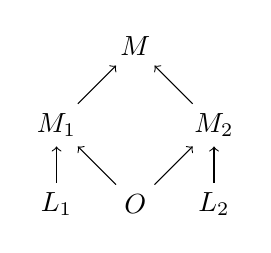
\begin{tikzpicture} %[scale=0.8]
    \node (o) at (0,0) {\(O\)};
    \node (n) at (0,2) {\(M\)};
    \node (l1) at (-1,0) {\(L_1\)};
    \node (l2) at (1,0) {\(L_2\)};
    \node (n1) at (-1,1) {\(M_1\)};
    \node (n2) at (1,1) {\(M_2\)};
    \draw [->] (l1) -- (n1);
    \draw [->] (l2) -- (n2);
    \draw [->] (o) -- (n1);
    \draw [->] (o) -- (n2);
    \draw [->] (n1) -- (n);
    \draw [->] (n2) -- (n);
  \end{tikzpicture}
  \]
  where $\labl(e_1)\redl{-}_O\labl(e_2)$, for some graph $O$.
\end{definition}

\subsection{From posets to traces}

\begin{lemma}
  \label{lem:rewrite_concurrent}
  Let $(E,\subseteq,\labl, \bp) $ be the refinement of a decorated poset and let $e_1,e_2\in E$ be two incomparable events such that
  $\bp(e_1) = M_1\overset{e_1}{\Rightarrow} M_1'$ and $\bp(e_2) = M_2\overset{e_2}{\Rightarrow} M_2'$.
  \begin{enumerate}
  \item if the two productions are co-initial, i.e. $M_1\iso M_2$ then there exists $M'$ such that the diagram commutes
  \[
  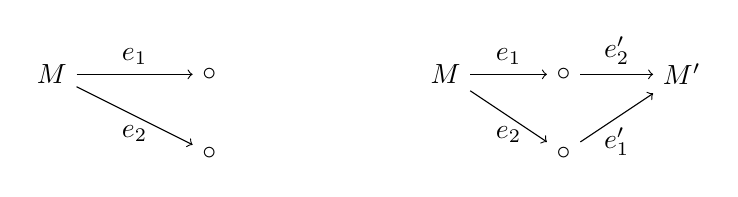
\begin{tikzpicture} %[scale=0.8]
    \node (m2) at (0,0) {\(\circ\)};
    \node (m1) at (0,1) {\(\circ\)};
    \node (m) at (-2,1) {\(M\)};
    \node (implies) at (2,1) {\(\implies\)};
    \node (mm2) at (4.5,0) {\(\circ\)};
    \node (mm1) at (4.5,1) {\(\circ\)};
    \node (n) at (6,1) {\(M'\)};
    \node (mm) at (3,1) {\(M\)};
    \draw [->] (m) -- node [left,above] {\(e_1\)} (m1);
    \draw [->] (m) -- node [left,below] {\(e_2\)} (m2);
    \draw [->] (mm) -- node [left,above] {\(e_1\)} (mm1);
    \draw [->] (mm) -- node [left,below] {\(e_2\)} (mm2);
    \draw [->] (mm1) -- node [left,above] {\(e_2'\)} (n);
    \draw [->] (mm2) -- node [left,below] {\(e_1'\)} (n);
  \end{tikzpicture}
  \]

  \item if the two productions are co-final, i.e. $M_1'\iso M_2'$ then there exists $M'$ such that the diagram commutes
  \[
  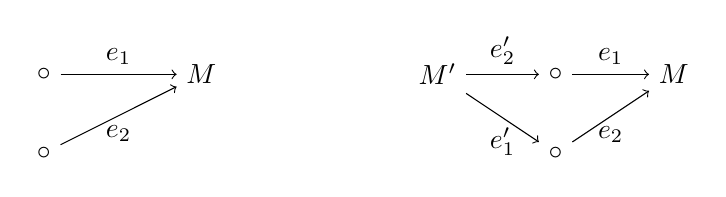
\begin{tikzpicture} %[scale=0.8]
    \node (m2) at (-2,0) {\(\circ\)};
    \node (m1) at (-2,1) {\(\circ\)};
    \node (m) at (0,1) {\(M\)};
    \node (implies) at (2,1) {\(\implies\)};
    \node (mm2) at (4.5,0) {\(\circ\)};
    \node (mm1) at (4.5,1) {\(\circ\)};
    \node (n) at (3,1) {\(M'\)};
    \node (mm) at (6,1) {\(M\)};
    \draw [->] (m1) -- node [left,above] {\(e_1\)} (m);
    \draw [->] (m2) -- node [left,below] {\(e_2\)} (m);
    \draw [->] (mm1) -- node [left,above] {\(e_1\)} (mm);
    \draw [->] (mm2) -- node [left,below] {\(e_2\)} (mm);
    \draw [->] (n) -- node [left,above] {\(e_2'\)} (mm1);
    \draw [->] (n) -- node [left,below] {\(e_1'\)} (mm2);
  \end{tikzpicture}
  \]
  \end{enumerate}
\end{lemma}
\begin{proof}
  \begin{enumerate}
  \item Let $\labl(e_1)=L_1\action R_1$ and $\labl(e_2)=L_2\action R_2$ be the labels of the two events.
    Then there exists an event $e_3$ such that $e_3\subseteq_{O_1} e_1$ and $e_3\subseteq_{O_2} e_2$. We can assume without loss of generality, that $e_3$ is the only such event (in the cover relation with $e_1$ and $e_2$). Let us show that we can rewrite $M_1'$ using rule $\labl(e_2)$ and obtain $M'$ such that $M_1\overset{e_1}{\Rightarrow} M_1'$ and $M_1'\overset{e_2'}{\Rightarrow} M_2'$ are sequentially independent.

     Let us consider only the poset restricted to events $\{e_1,e_2,e_3\}$. We have that, in the following diagram, there exists a morphism $L_2\to D'$ that commutes.
     \[
     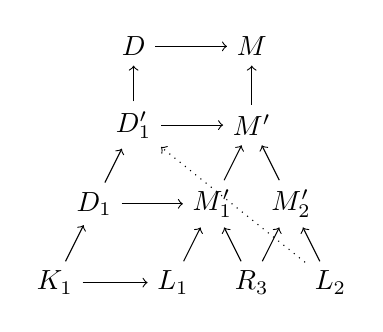
\begin{tikzpicture} %[scale=0.8]
       \node (k1) at (0,0) {\(K_1\)};
       \node (l1) at (1.5,0) {\(L_1\)};
       \node (r3) at (2.5,0) {\(R_3\)};
       \node (l2) at (3.5,0) {\(L_2\)};
       \node (m1) at (2,1) {\(M_1'\)};
       \node (m2) at (3,1) {\(M_2'\)};
       \node (d1) at (0.5,1) {\(D_1\)};
       \node (d1p) at (1,2) {\(D_1'\)};
       \node (m1p) at (2.5,2) {\(M'\)};
       \node (d) at (1,3) {\(D\)};
       \node (m) at (2.5,3) {\(M\)};
       \draw [->] (k1) -- (l1);
       \draw [->] (k1) -- (d1);
       \draw [->] (d1) -- (d1p);
       \draw [->] (d1) -- (m1);
       \draw [->] (d1p) -- (d);
       \draw [->] (d1p) -- (m1p);
       \draw [->] (d) -- (m);
       \draw [->] (l1) -- (m1);
       \draw [->] (r3) -- (m1);
       \draw [->] (r3) -- (m2);
       \draw [->] (l2) -- (m2);
       \draw [->] (m2) -- (m1p);
       \draw [->] (m1) -- (m1p);
       \draw [->] (m1p) -- (m);
       \draw [dotted,->] (l2) -- (d1p);
     \end{tikzpicture}
     \]

     Using the corollar of~\autoref{lem:subposet} if there is no such morphism then events are sequential dependent in the original trace. From~\autoref{def:abstraction}, one has that $e_1 < e_2$, which contradicts the hypothesis.

     If there exists a morphism $L_2\to D'$ that commutes then, using~\autoref{lem:subposet} there is a morphism from $L_2\to D$ that commutes.
     Lastly we use~\autoref{church_rosser} which from such a morphism, infers that $M\overset{e_1}{\Rightarrow} M_1'$ and $M\overset{e_2}{\Rightarrow} M_2'$ are parallel independent.

  \item As we are using DPO rewriting, this case is similar to the first.
  \end{enumerate}
\end{proof}


\begin{definition}[Concretisation of a poset]
  \label{def:concretisation}
  Given a set of posets $\mathcal{S}$ let us define the concretisation function $\gamma:\mathcal{S}\subseteq\Theta$ that sends a poset to a set of traces.
  \begin{itemize}
  \item For $s\in\mathcal{S}$, let $\overline{s}\in\mathit{decorate}(s)$ be a decorated poset.
    We define the refinement of a decorated poset $\mathit{refine}(\overline{s}) = \{E,\sqsubset,\labl,\bp\}$, where $\overline{s} = \{E,\sqsubset,\labl\}$.
  \item For every pair of concurrent events in $\mathit{refine}(\overline{s})$ close out the diagram using~\autoref{lem:rewrite_concurrent}. Denote $S$ a diagram that is closed with respect to the concurrent events. Then define $\gamma$, the concretisation function, as a set of traces, where each trace is a path in the diagram $S$:
    \[
    \gamma(s) = \{ t : t\text{ is a path in }S\text{ and }S\text{ is one the closed diagrams of }\mathit{refine}(\mathit{decorate}(s))\}.
    \]
  \end{itemize}
\end{definition}

\begin{example}
  We complete the refined poset of the left by applying~\autoref{lem:rewrite_concurrent} to obtain the diagram on the right:
  \[
  \begin{tikzpicture} %[scale=0.8]
  \node (n2) at (-1,1) {\(\circ\)};
  \node (m2) at (0,0) {\(\circ\)};
  \node (m1) at (0,1) {\(\circ\)};
  \node (n) at (1,1) {\(\circ\)};
  \node (implies) at (2,1) {\(\leadsto\)};
  \node (mm2) at (5.6,0) {\(\circ\)};
  \node (mm1) at (5.6,1) {\(\circ\)};
  \node (nn) at (6.9,1) {\(\circ\)};
  \node (mm) at (4.3,0) {\(\circ\)};
  \node (nn1) at (3,0) {\(\circ\)};
  \node (nn2) at (4.3,1) {\(\circ\)};
  \node (text) at (0.8,0.4) {\(e_3\)};
  \node (text1) at (5.3,0.5) {\(e_3'\)};
  \draw [->] (n2) -- node [left,above] {\(e_1\)} (m1);
  \draw [->] (m1) -- node [left,above] {\(e_2\)} (n);
  \draw [->] (m2) -- (n);
  \draw [->] (nn2) -- node [left,above] {\(e_1\)} (mm1);
  \draw [->] (mm1) -- node [left,above] {\(e_2\)} (nn);
  \draw [->] (mm2) -- node [left,below] {\(e_3\)} (nn);
  \draw [->] (mm) -- node [left,below] {\(e_2'\)} (mm2);
  \draw [->] (mm) -- (mm1);
  \draw [->] (nn1) -- node [above] {\(e_3''\)} (nn2);
  \draw [->] (nn1) -- node [left,below] {\(e_1'\)} (mm);
\end{tikzpicture}
\]
\end{example}

%% \[
%% \begin{tikzpicture} %[scale=0.8]
%%   \node (m2) at (0,0) {\(\circ\)};
%%   \node (m1) at (0,1) {\(\circ\)};
%%   \node (n) at (1,1) {\(\circ\)};
%%   \node (n1) at (2,1) {\(\circ\)};
%%   \node (n2) at (2,0) {\(\circ\)};
%%   \node (implies) at (3,1) {\(\leadsto\)};
%%   \node (m) at (4,1) {\(\circ\)};
%%   \node (mm2) at (5,0) {\(\circ\)};
%%   \node (mm1) at (5,1) {\(\circ\)};
%%   \node (nn) at (6,1) {\(\circ\)};
%%   \node (nn1) at (7,1) {\(\circ\)};
%%   \node (nn2) at (7,0) {\(\circ\)};
%%   \node (p) at (8,1) {\(\circ\)};
%%   \draw [->] (n) -- node [left,above] {\(e_3\)} (n1);
%%   \draw [->] (n) -- node [left,below] {\(e_4\)} (n2);
%%   \draw [->] (m1) -- node [left,above] {\(e_1\)} (n);
%%   \draw [->] (m2) -- node [left,below] {\(e_2\)} (n);
%%   \draw [->] (nn) -- node [left,above] {\(e_3\)} (nn1);
%%   \draw [->] (nn) -- node [left,below] {\(e_4\)} (nn2);
%%   \draw [->] (mm1) -- node [left,above] {\(e_1\)} (nn);
%%   \draw [->] (mm2) -- node [left,below] {\(e_2\)} (nn);
%%   \draw [->] (m) -- node [left,above] {\(e_2'\)} (mm1);
%%   \draw [->] (m) -- node [left,below] {\(e_1'\)} (mm2);
%%   \draw [->] (nn1) -- node [left,above] {\(e_3'\)} (p);
%%   \draw [->] (nn2) -- node [left,below] {\(e_4'\)} (p);
%% \end{tikzpicture}
%% \]
%% \[
%% \begin{tikzpicture} %[scale=0.8]
%%   \node (m) at (-1,1) {\(\circ\)};
%%   \node (m2) at (0,0) {\(\circ\)};
%%   \node (m1) at (0,1) {\(\circ\)};
%%   \node (n) at (1,1) {\(\circ\)};
%%   \node (implies) at (2,1) {\(\leadsto\)};
%%   \node (implies2) at (7,1) {\(~\)};
%%   \draw [->] (m) -- node [left,above] {\(e_1\)} (m1);
%%   \draw [->] (m) -- node [left,below] {\(e_2\)} (m2);
%%   \draw [->] (m1) -- node [left,above] {\(e_3\)} (n);
%%   \draw [->] (m2) -- node [left,below] {\(e_4\)} (n);
%% \end{tikzpicture}
%% \]

\begin{lemma}
  $\theta\subseteq \gamma(\alpha(\theta))$.
\end{lemma}
\begin{proof}
    \begin{mdframed}[backgroundcolor=blue!20]
    to do
  \end{mdframed}
\end{proof}

\begin{remark}[Adding inhibition]
  We can change definition~\autoref{def:abstraction} in order to construct posets with the additional relation of inhibition between events:
  \[
  e_i \dashv e_j \iff t_i \dashv t_j \text{ and } \alpha(t_i)=e_i, \alpha(t_j)=e_j
  \]
  Inhibition doesn't change the decoration and refinement of a poset but can make the concretisation function "more precise". In~\autoref{def:concretisation} we have to additionally remove any path in $\gamma(\alpha(\theta))$ that has two events $e_1$ followed by $e_2$ such that $e_1\dashv e_2$.
\end{remark}
